\section{Durchführung}
\label{sec:Durchführung}
Der Aufbau dieses Versuches besteht im Wesentlichen aus einer transparenten Grundplatte, auf welcher zwei verschiebbare Laser mit Wellenlängen $\lambda_\text{rot} =
\qty{635}{\nano\metre}$ und $\lambda_\text{grün} = \qty{532}{\nano\metre}$ montiert sind.
Durch die Transparenz der Platte lassen sich Papiervorlagen mit Winkelskalen unterlegen, die die Auswertung der verschiedenen Teilversuche vereinfachen.
Die Grundplatte und elementare Bauteile sind in \autoref{fig:Aufbau} zu sehen.

\begin{figure}
  \centering
  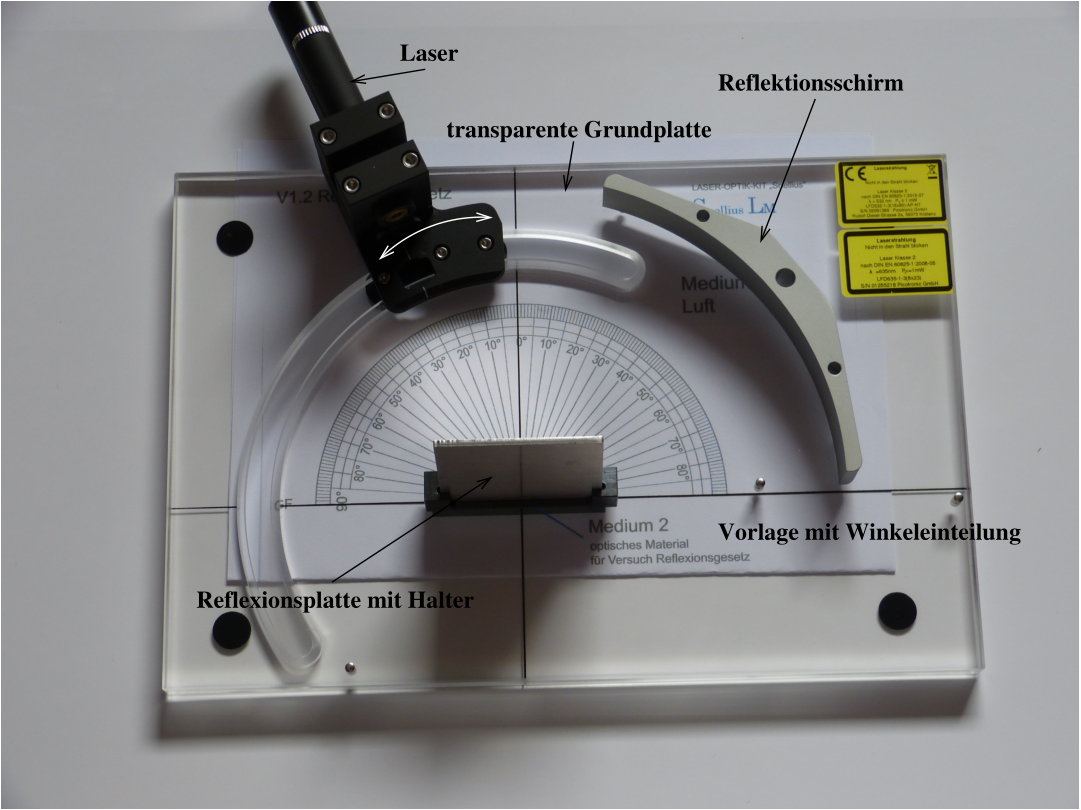
\includegraphics[width=0.7\textwidth]{content/Platte.png}
  \caption{Im Versuch verwendete Grundplatte. Zu sehen sind die Laser, eine Spiegelhalterung, der Reflexionsschirm und eine Papiervorlage zur Winkelmessung \cite{v400}.}
  \label{fig:Aufbau}
\end{figure}
  
Auf dieser Grundplatte können ein Spiegel, ein Prisma, eine planparallele Platte und verschiedene Gitter installiert werden, die in den folgenden Teilversuchen verwendet werden.

\subsection{Messaufgabe 1: Reflexionsgesetz}
\label{subsec:D_Reflexion}
Für den ersten Teilversuch wird der grüne Laser und ein Spiegel, sowie die Papiervorlage A verwendet. Der Laser wird in 7 verschiedenen Einfallswinkeln $\alpha_1$ 
zum Lot der Reflexionsfläche eingestellt. Die Ausfallswinkel $\alpha_2$ können ebenfalls an einer Skala abgelesen werden. Die jeweiligen Winkel werden notiert. 
Es sollte darauf geachtet werden, den Spiegel in der korrekten Ausrichtung
einzusetzen, um systematische Fehler der Messung zu verhindern. Die Messwerte können mit der Theorieerwartung \dq Einfallswinkel = Ausfallswinkel\dq \; verglichen werden.

\subsection{Messaufgabe 2: Brechungsgesetz}
\label{subsec:D_Brechung}
Zur Überprüfung des Brechungsgesetzes wird die planparallele Platte verwendet. Bei korrekter Platzierung dieser, kann der Winkel $\beta$ des gebrochenen Lichtsrahls direkt an Hinterseite
der planparallelen Platte abgelesen werden. Es werden zu 7 Einfallswinkeln Messwerte des Brechungswinkels genommen. Aus den Messwerten kann der Brechungsindex $n$ und die
Lichtgeschwindigkeit im Material der Platte (Plexiglas) bestimmt werden. Außerdem kann der Strahlenversatz mithilfe der Formel \ autoref{eqn:WasWeißIch} berechnet werden.
Der Winkel $\beta$ kannd dabei sowohl experimentell abgelesen, als auch über das Brechungsgesetz bestimmt werden. Die beiden Ergebnisse der unterschiedlichen Methoden werden 
verglichen.

\subsection{Messaufgabe 3: Brechung im Prisma}
\label{subsec:D_Prisma}
Für diesen Versuchsteil wird die Papiervorlage C und das Prisma verwendet. Außerdem werden die Messungen für den grünen- und roten Laser durchgeführt.
Das Prisma wird in der Mitte der Grundplatte befestigt. Für 7 verschiedene Einfallswinkel $\alpha_1$ werden die Austrittswinkel $\alpha_2$ bestimmt. Die Winkel
sollten dabei in einem Bereich von $\qty{10}{\degree}$ bis $\qty{60}{\degree}$ gewählt werden. Aus den Messwerten kann die Ablenkung $\delta$ mithilfe des Brechungsindizes 
von Kronglas bestimmt werden.

\subsection{Messaufgabe 4: Beugung am Gitter}
\label{subsec:D_Beugung}
Für diesen Versuch wird eine Halterung mit verschiedenen Beugungsgittern verwendet. Es wird eine geeignete Winkelskala hinter der Grundplatte aufgebaut. An der Seite der
Grundplatte, die dem Laser gegenüber steht, kann eine Halterung mit verschiedenen Beugungsgittern platziert werden. Nachdem der Laser so justiert ist, dass er ohne Beugungsgitter
genau den Nullpunkt der Skala trifft, können die verschiedenen Beugungsgitter eingesetzt werden.
Es entsteht ein Beugungsbild, an welchem Ordnungen der Beugung und zugehörige Winkel abgelesen werden können. Mithilfe dieser kann ein experimenteller Wert 
der Wellenlängen der beiden Laser bestimmt werden. Dieses Vorgehen wird für alle drei Gitter durchgeführt.

\subsection{Vorbereitungsaufgaben}
\label{subsec:Vorbereitung}
Vor der Durchführung des Versuches sollen einige Literaturwerte von Brechungsindizes festgestellt werden. Diese sind in \autoref{tab:Brechungsindizes} aufgeführt.

\begin{table}
    \centering
    \caption{Brechungsindizes verschiedener Materialien. \cite{czichos}}
    \label{tab:Brechungsindizes}
    \begin{tabular}{c S[table-format = 1.5]}
        \toprule
        {Material} & {Brechungsindex $n$} \\
        \midrule
        {Luft}      & {1,00029} \\ 
        {Wasser}    &  {1,3304} \\  
        {Kronglas}  &  {1,5067} \\ 
        {Plexiglas} &   {1.489} \\ 
        {Diamant}   &  {2,4173} \\ 
        \bottomrule
    \end{tabular}
  \end{table}
  
Des Weiteren gilt es die Gitterkonstanten verschiedener Gitter zu berechnen. Diese sind \autoref{tab:Gitter} zu entnehmen.

  \begin{table}[H]
    \centering
    \caption{Gitterkonstanten für Gitter mit 600, 300, und 100 Linien pro Millimeter.}
    \label{tab:Gitter}
    \begin{tabular}{S[table-format = 3.0] c}
        \toprule
        {Linien\,/\,mm} & {$d \mathbin{/} \unit{\micro\metre}$} \\
        \midrule
        600 & 1,667 \\
        300 & 3,333 \\
        100 & 10    \\ 
        \bottomrule
    \end{tabular}
  \end{table}
